\documentclass[12pt]{article}
\usepackage[utf8]{inputenc}
\usepackage[english]{babel}
\usepackage{amsmath}
\usepackage{amssymb}
\usepackage{bm}
\usepackage{listings}
\usepackage{minted}
\usepackage{graphicx}
\usepackage{subfig}

\graphicspath{./images/}
\setlength\parindent{0pt} % Removes all indentation from paragraphs
\newcommand{\uvec}[1]{\boldsymbol{\hat{\textbf{#1}}}}
\title{ECE421 - Winter 2021 \\ Neural Networks}
\author{Shayshu Nahata-Ragubance}
\date{\today}
\begin{document}
\maketitle

\section{Objective}
Implement a 3 layer fully connected neural network using numpy.
The architecture is given as the following:
\begin{itemize}
  \item Input layer: 28 by 28 image
  \item Hidden layer: $\mathbf{h} = ReLU(\mathbf{W}_h + \mathbf{b}_h)$
  \item Output: $\mathbf{p} = softmax(\mathbf{o})$, where $\mathbf{o} = \mathbf{W}_o \mathbf{h} + \mathbf{b}$
\end{itemize}

\section{Neural Networks using Numpy}

\subsection{Helper Functions}
For this section several helper function were created to aid with forward, and backpropagation.
One note is that in the softmax function, the maximum value of the input matrix is subtracted from
each element in order to prevent logical overflow.
Shown below is the analytical expression of $\frac{\partial \mathcal{L}}{\partial \mathbf{o}}$:
\begin{equation}
  \begin{split}
    \frac{\partial \mathcal{L}}{\partial \mathbf{o}} & = \frac{\partial \mathcal{L}}{\partial \sigma(\mathbf{o})} \cdot \frac{\partial \sigma(\mathbf{o})}{\partial \mathbf{o}} \\
    & = - \mathbf{y} \cdot \frac{1}{\sigma (\mathbf{o})} \cdot \sigma (\mathbf{o}) \cdot (1 - \sigma (\mathbf{o})) \\
    & = \sigma (\mathbf{o}) - \mathbf{y}
  \end{split}
\end{equation}
\begin{description}
  \item{ReLU}
        \begin{minted}{python}
        def relu(x):
            return np.maximum(0, x)
        \end{minted}
  \item{Softmax}
        \begin{minted}{python}
        def softmax(x):
            x = x - np.max(x)
            return np.exp(x) / np.sum(np.exp(x), axis=1, keepdims=True)
        \end{minted}
  \item{Compute}
        \begin{minted}{python}
        def compute(X, W, b):
            return np.add(np.matmul(X, W), b)
    \end{minted}
  \item{Average Cross entropy}
        \begin{minted}{python}

        def averageCE(y, y_hat):
            log_pred = np.log(y_hat)

            return -1 * np.mean(y * log_pred)
    \end{minted}
  \item{Gradient Cross entropy loss}
        \begin{minted}{python}
        def gradCE(targets, input):
            return softmax(input) - targets
        \end{minted}
\end{description}


\subsection{Backpropagation Derivation}
To train the neural networks partial derivatives of the loss function with respect to differnt
variables is needed in order to implement backpropagation and eventually gradient descent.
Shown below is the derivation of the necessary partial derivatives:
\begin{description}
  \item{Loss with respect to output weights}
        \begin{equation}
          \begin{aligned}
            \frac{\partial \mathcal{L}}{\partial \mathbf{W}_o} & = \frac{\partial \mathcal{L}}{\partial \sigma (\mathbf{o})} \cdot \frac{\partial \sigma(\mathbf{o})}{\partial \mathbf{o}} \cdot \frac{\partial \mathbf{o}}{\partial \mathbf{W}_o} \\
                                                               & = (\sigma (\mathbf{o}) - \mathbf{y}) \mathbf{h}                                                                                                                                   \\
                                                               & = \mathbf{h}^T (\sigma (\mathbf{W}_{o} \mathbf{h} + \mathbf{b}_o) - \mathbf{y})
          \end{aligned}
        \end{equation}
  \item{Loss with respect to output bias}
        \begin{equation}
          \begin{aligned}
            \frac{\partial \mathcal{L}}{\partial \mathbf{b}_o} & = \frac{\partial \mathcal{L}}{\partial \mathbf{o}} \cdot \frac{\partial\mathbf{o}}{\partial \mathbf{b}_o} \\
                                                               & = \sigma (\mathbf{W}_{o} \mathbf{h} + \mathbf{b}_o) - \mathbf(y)
          \end{aligned}
        \end{equation}
  \item{Loss with respect to hidden weights}
        \begin{equation}
          \begin{aligned}
            \frac{\partial \mathcal{L}}{\partial \mathbf{W}_h} = \frac{\partial \mathcal{L}}{\partial \mathbf{o}} \cdot \frac{\partial \mathbf{o}}{\partial \mathbf{h}} \cdot \frac{\partial \mathbf{h}}{\partial \mathbf{s}_i} \cdot \frac{\partial \mathbf{s}_i}{\partial \mathbf{W}_h} \\
            \frac{\partial \mathcal{L}}{\partial \mathbf{o}} = \sigma (\mathbf{W}_{o} \mathbf{h} + \mathbf{b}_o) - \mathbf(y)                                                                                                                                                             \\
            \frac{\partial \mathbf{o}}{\partial \mathbf{h}} = \mathbf{W}_o^T                                                                                                                                                                                                              \\
            \frac{\partial \mathbf{h}}{\partial \mathbf{s}_i} = \begin{cases}
              1 & \mathbf{W}_{hi} \mathbf{x}_i + \mathbf{b}_{hi} > 0 \\
              0 & Otherwise
            \end{cases}                                                                                                                                                                                                 \\
            \frac{\partial \mathbf{s}_i}{\partial \mathbf{W}_h} = \mathbf{x}                                                                                                                                                                                                              \\
            \textrm{This means that for every element in the matrix }
            \mathbf{W}_{o} \mathbf{h} + \mathbf{b}_o                                                                                                                                                                                                                                      \\
            \textrm{check if that element is greater than 0, if it is than add it}                                                                                                                                                                                                        \\
            \textrm{to the respective position in the matrix}                                                                                                                                                                                                                             \\                                                                                                                                    \\
            \therefore \frac{\partial \mathcal{L}}{\partial \mathbf{W}_h} = \mathbf{x} [(\mathbf{W}_{h} \mathbf{x} + \mathbf{b}_{h}) \otimes \frac{\partial \mathbf{h}}{\partial \mathbf{s}_i}] [(\sigma (\mathbf{W}_{o} \mathbf{h} + \mathbf{b}_o) - \mathbf{y}) \mathbf{W}_o^T]         \\
          \end{aligned}
        \end{equation}
  \item{Loss with respect to hidden bias}
        \begin{equation}
          \begin{aligned}
            \frac{\partial \mathcal{L}}{\partial \mathbf{b}_h} = \frac{\partial \mathcal{L}}{\partial \mathbf{o}} \cdot \frac{\partial \mathbf{o}}{\partial \mathbf{h}} \cdot \frac{\partial \mathbf{h}}{\partial \mathbf{s}_i} \cdot \frac{\partial \mathbf{s}_i}{\partial \mathbf{b}_h} \\
            \frac{\partial \mathbf{o}}{\partial \mathbf{h}} = \mathbf{W}_o^T                                                                                                                                                                                                              \\
            \frac{\partial \mathbf{h}}{\partial \mathbf{s}_i} = \begin{cases}
              1 & \mathbf{W}_{hi} \mathbf{x}_i + \mathbf{b}_{hi} > 0 \\
              0 & Otherwise
            \end{cases}                                                                                                                                                                                                 \\
            \therefore \frac{\partial \mathcal{L}}{\partial \mathbf{b}_h} = \mathbf{J}_{1000} \otimes \frac{\partial \mathbf{h}}{\partial \mathbf{b}_h} [(\sigma (\mathbf{W}_{o} \mathbf{h} + \mathbf{b}_o) - \mathbf{y}) \mathbf{W}_o^T]                                                 \\
            \textrm{Where } \mathbf{J} \textrm{ is a matrix of ones}                                                                                                                                                                                                                      \\
          \end{aligned}
        \end{equation}
\end{description}
\subsection{Learning}
Shown below is the code used to train the neural network, along with any necessary helper functions used.

\begin{minted}{python}
def intiWeights(sizes):
  scale_1 = np.sqrt((2.0 / (sizes[0][0] + sizes[0][1])))
  scale_2 = np.sqrt((2.0 / (sizes[1][0] + sizes[1][1]))) 

  Wh = np.random.normal(loc=0.0, scale=scale_1, size=sizes[0])
  Wo = np.random.normal(loc=0.0, scale=scale_2, size=sizes[1])
  return Wh, Wo
\end{minted}

\begin{minted}{python}
def initBias(sizes):
  bo = np.zeros((sizes[0][0], sizes[0][1]))
  bh = np.zeros((sizes[1][0], sizes[1][1]))
  return bo, bh
\end{minted}

\begin{minted}{python}
def initMomentum(sizes, value):
  vWh = np.full(sizes[0], value)
  vWo = np.full(sizes[1], value) 
  vbh = np.zeros(sizes[2]) 
  vbo = np.zeros(sizes[3])
  return vWh, vWo, vbh, vbo 
\end{minted}

\begin{minted}{python}
def backProp(x0, x1, x2, s1, s2, Wh, Wo, bh, bo, y):
  # dl_do = softmax(s2) - y
  dL_do = ( 1.0/ 10000 ) * gradCE(y, s2)

  # # dL_dWo = x2^T * (softmax(s2) - y)
  dL_dWo = np.matmul(np.transpose(s1), dL_do)

  # dL_dbo = (softmax(s2) - y) but in the right shape...
  dL_dbo = np.matmul(np.ones((1, y.shape[0])), dL_do)

  # dL_dWh = x0 * pw(Relu) *(softmax(s2) - y) * W^T
  ds1_dx1 = np.where(s1 > 0, 1, 0)
  dL_dWh = np.matmul(dL_do, np.transpose(Wo))
  dL_dWh = np.matmul(np.transpose(x0), ds1_dx1 * dL_dWh)

  # dL_dbh = pw(Relu) * (softmax(s2) - y) * W^T
  dL_dbh = np.matmul(dL_do, np.transpose(Wo))
  dL_dbh = np.where(s1 > 0, dL_dbh, 0)
  dL_dbh = np.matmul(np.ones((1, s1.shape[0])), dL_dbh)
 
  return dL_dWo, dL_dbo, dL_dWh, dL_dbh 
\end{minted}

\begin{minted}{python}
def newMomentum(vold, dL_dx, alpha=0.1, gamma=0.9):
  vWh = (gamma * vold[0]) + (alpha * dL_dx[0])
  vWo = (gamma * vold[1]) + (alpha * dL_dx[1]) 
  vbh = (gamma * vold[2]) + (alpha * dL_dx[2]) 
  vbo = (gamma * vold[3]) + (alpha * dL_dx[3]) 

  return vWh, vWo, vbh, vbo 
\end{minted}

\begin{minted}{python}
def gradientDescent(Wh_old, Wo_old, bh_old, bo_old, vWh, vWo, vbh, vbo):
  Wh = Wh_old - vWh
  Wo = Wo_old - vWo
  bh = bh_old - vbh
  bo = bo_old - vbo
  
  return Wh, Wo, bh, bo
\end{minted}

\begin{minted}{python}
def accuracy(prediction, target):
  y_hat = np.argmax(prediction, axis = 1)
  y = np.argmax(target, axis = 1)

  result = np.equal(y, y_hat)
  accuracy = np.sum(result) / target.shape[0]
  
  return accuracy
\end{minted}

\begin{minted}{python}
def train(epochs=10, learning_rate=0.1, momentum=0.9):
  # Get the data and reshape it...
  trainData, validData, testData, trainTarget, \\
    validTarget, testTarget = loadData()

  trainTarget, validTarget, testTarget \\
    = convertOneHot(trainTarget, validTarget, testTarget)

  trainData = trainData.reshape((trainData.shape[0], -1))
  validData = validData.reshape((validData.shape[0], -1))
  testData = testData.reshape((testData.shape[0], -1))

  # Intitialize weights, bias, and descent...
  bo, bh = initBias([(1, 10), (1, 1000)])
  Wh, Wo = intiWeights([(784, 1000), (1000, 10)])
  vWh, vWo, vbh, vbo = \\
    initMomentum([(784, 1000), (1000, 10), (1, 1000), (1, 10)], 1e-5)

  # Loss and accuracy variables...
  itters = []
  train_loss, val_loss, test_loss = [], [], []
  train_acc, val_acc, test_acc = [], [], []


  for itteration in range(epochs):
    # Compute forward propagation for the training set...
    s1 = compute(trainData, Wh, bh)
    x1 = relu(s1)

    s2 = compute(x1, Wo, bo)
    x2 = softmax(s2)

    # Compute forward propagation for the validation set...
    val_s1 = compute(validData, Wh, bh)
    val_x1 = relu(val_s1)

    val_s2 = compute(val_x1, Wo, bo)
    val_x2 = softmax(val_s2)

    # Compute forward propagation for the testing set...
    test_s1 = compute(testData, Wh, bh)
    test_x1 = relu(test_s1)

    test_s2 = compute(test_x1, Wo, bo)
    test_x2 = softmax(test_s2)

    # Calculate the loss and accuracy for the training set...
    train_loss.append(averageCE(trainTarget, x2))
    train_acc.append(accuracy(x2, trainTarget))

    # Calculate the loss and accuracy for the validation set...
    val_loss.append(averageCE(validTarget, val_x2))
    val_acc.append(accuracy(val_x2, validTarget))

    # Calculate the loss and accuracy for the testing set...
    test_loss.append(averageCE(testTarget, test_x2))
    test_acc.append(accuracy(test_x2, testTarget))

    # Compute back propagation...
    # Use the formulas developed in 1.2 to compute the gradient of 
    # the loss function with respect to Wo, bo, Wh, and bh....
    dL_dWo, dL_dbo, dL_dWh, dL_dbh = \\
        backProp(trainData, x1, x2, s1, s2, Wh, Wo, bh, bo, trainTarget)

    # Now get the new momentum/descent terms using the 
    #  partial derivatives calculated...
    vWh, vWo, vbh, vbo = \\
        newMomentum([vWh, vWo, vbh, vbo], \\
        [dL_dWh, dL_dWo, dL_dbh, dL_dbo], \\
         alpha=learning_rate, gamma=momentum)

    # Compute the new values of the weights and bias 
    # using gradient descent
    Wh, Wo, bh, bo = \\
        gradientDescent(Wh, Wo, bh, bo, vWh, vWo, vbh, vbo)

    itters.append(itteration)

  return train_loss, val_loss, test_loss, train_acc, \\
    val_acc, test_acc, itters
\end{minted}

The results from training are shown in the graph and table below. In summary
this model was able to achieve a 96\% accuracy on the training set and a 90\% 
accuracy on the validation set. In the future this value can most likely be increased by adjusting
hyperparameters such as learning rate, and by implementing modifications such as drop out.
\begin{center}
  \begin{table}[h]
    \centering
    \begin{tabular}{||c c c c||}
      \hline
      Metric   & Train   & Validation & Test   \\
      \hline\hline
      Accuracy & 0.9690  & 0.9072     & 0.9079 \\
      \hline
      Loss     & 0.01400 & 0.03275    & 0.0355 \\
      \hline
    \end{tabular}
    \caption{\label{tab: table-name}Best accuracy and loss for each dataset}
  \end{table}
\end{center}

\begin{figure}[h]
  \centering
  \subfloat{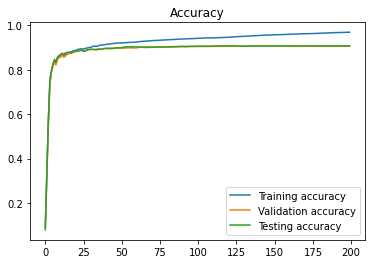
\includegraphics{images/ANN_acc.png}}
  \caption{Accuracy graph for neural network}
\end{figure}

\begin{figure}
  \centering
  \subfloat{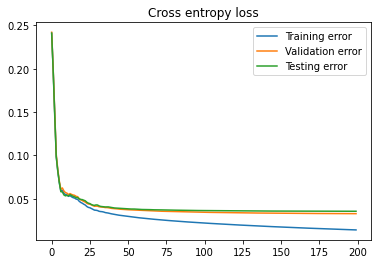
\includegraphics{images/ANN_loss.png}}
  \caption{Loss graph for neural network}
\end{figure}


\end{document}